% !TeX root = ../main.tex

\chapter{Appendix}

\section{Appendix}

\subsection{Detailed Monte Carlo and Data Samples}
\label{subsec:samples_zz}

This section provides comprehensive lists of dataset identifiers (DSIDs), cross-sections, and generation parameters for the Monte Carlo simulated samples, as well as the exact trigger chains and Good Run Lists (GRLs) utilized in the main analysis (Section~\ref{sec:llvv_samples}).

\begin{table}[htbp]
\centering
\scriptsize
\begin{tabularx}{400pt}{|X||c|c|c|c|}
\hline
\centering \textbf{Process} & \textbf{DSID} & \textbf{Generator} & \textbf{$\sigma$ [pb]} & \textbf{k-factor}\\
\hline
\centering $gg\rightarrow ZZ \to \ell^+\ell^-\nu\bar{\nu}$ & 345723 & Sherpa 2.2.2 & 0.0071108 & 1.7 \\ \hline
\centering $q\bar{q}\rightarrow ZZ/\gamma^* \to \ell^+\ell^-\nu\bar{\nu}$ & 345666 & Sherpa 2.2.2 & 0.49908 & 1.5 \\ \hline
\centering Electroweak $ZZjj \to \ell^+\ell^-\nu\bar{\nu}jj$ & 363724 &  MadGraph5 & 0.0013529 & - \\ \hline
\end{tabularx}
\caption{\rm Summary of Monte Carlo samples used to model the SM $ZZ \to \ell^+\ell^-\nu\bar{\nu}$ signal components.}
\label{tab:ZZ_signal_samples}
\end{table}

\begin{table}[htbp]
\centering
\scriptsize
\begin{tabularx}{400pt}{|X|c|}
\hline
\centering \textbf{Process} & \textbf{DSID} \\
\hline
nunull\_f4gamma\_plus0001 & 367911 \\ \hline
nunull\_f4Z\_plus0001 & 367912 \\ \hline
nunull\_f5gamma\_plus0001 & 367913 \\ \hline
nunull\_f5Z\_plus0001 & 367914 \\ \hline
nunull\_sm & 367915 \\ \hline
\end{tabularx}
\caption{\rm List of samples generated for the study of anomalous Neutral Triple Gauge Couplings (nTGCs).}
\label{tab:ZZEFTsamples}
\end{table}

\begin{table}[htbp]
\centering
\scriptsize
\begin{tabularx}{400pt}{|X|c|}
\hline
\centering \textbf{Process} & \textbf{DSID} \\
\hline
aQGCFT0\_INT\_05\_ZZ\_llvv & 515527 \\ \hline
aQGCFT0\_QUAD\_05\_ZZ\_llvv & 515528 \\ \hline
aQGCFT1\_INT\_1\_ZZ\_llvv & 515529 \\ \hline
aQGCFT1\_QUAD\_1\_ZZ\_llvv & 515530 \\ \hline
aQGCFT2\_INT\_1\_ZZ\_llvv & 515531 \\ \hline
aQGCFT2\_QUAD\_1\_ZZ\_llvv & 515532 \\ \hline
aQGCFT5\_INT\_1\_ZZ\_llvv & 515533 \\ \hline
aQGCFT5\_QUAD\_1\_ZZ\_llvv & 515534 \\ \hline
aQGCFT6\_INT\_1\_ZZ\_llvv & 515535 \\ \hline
aQGCFT6\_QUAD\_1\_ZZ\_llvv & 515536 \\ \hline
aQGCFT7\_INT\_1\_ZZ\_llvv & 515537 \\ \hline
aQGCFT7\_QUAD\_1\_ZZ\_llvv & 515538 \\ \hline
aQGCFT8\_INT\_1\_ZZ\_llvv & 515539 \\ \hline
aQGCFT8\_QUAD\_1\_ZZ\_llvv & 515540 \\ \hline
aQGCFT9\_INT\_2\_ZZ\_llvv & 515541 \\ \hline
aQGCFT9\_QUAD\_2\_ZZ\_llvv & 515542 \\ \hline
\end{tabularx}
\caption{\rm List of samples generated for the study of anomalous Quartic Gauge Couplings (aQGCs).}
\label{tab:ZZaQGCsamples}
\end{table}

\begin{table}[htbp]
\centering
\scriptsize
\begin{tabularx}{400pt}{|X||c|c|c|c|}
\hline
\centering \textbf{Process} & \textbf{DSID} & \textbf{Generator} & \textbf{$\sigma$ [pb]} & \textbf{k-factor}\\
\hline
\centering $gg\rightarrow ZZ \to 4\ell$ & 345706 & Sherpa 2.2.2 & 0.010091 & 1.7 \\ \hline 
\centering $q\bar{q}\rightarrow ZZ/\gamma^* \to 4\ell$ & 364250 & Sherpa 2.2.2 & 1.2522 & - \\ \hline 
\centering $q\bar{q}\rightarrow ZZ \rightarrow q\bar{q} \ell^+\ell^-$ & 363356 & Sherpa 2.2.1 & 15.565 & 0.1419 \\ \hline 
\end{tabularx}
\caption{\rm Summary of $ZZ$ background samples, including the four-lepton final state.}
\label{tab:ZZbkg_samples}
\end{table}

\begin{table}[htbp]
\centering
\scriptsize
\begin{tabularx}{400pt}{|X||c|c|c|c|}
\hline
\centering \textbf{Process} & \textbf{DSID} & \textbf{Generator} & \textbf{$\sigma$ [pb]} & \textbf{k-factor}\\
\hline
\centering $WZ \to \ell\nu\ell^+\ell^-$ & 364253 & Sherpa 2.2.2 & 4.5718 & - \\ \hline
\centering $WZjj \to \ell\nu\ell^+\ell^-jj$ & 364284 & Sherpa 2.2.2 & 0.047385 & - \\ \hline
\centering $WZ \rightarrow q\bar{q}\ell^{+} \ell^{-}$ & 363358 & Sherpa 2.2.1 & 3.4328 & - \\ \hline
\centering $q\bar{q} \rightarrow WW \to \ell\nu\ell\nu$ & 361600 & Powheg+Pythia8 & 10.631 & - \\ \hline
\centering $q\bar{q}\rightarrow WW \rightarrow q\bar{q} \ell\nu $ & 361606 & Powheg+Pythia8 & 44.18 & - \\ \hline
\centering $gg \rightarrow WW \to \ell\nu\ell\nu$ & 345718 & Sherpa 2.2.2 & 0.4823 & - \\ \hline
\end{tabularx}
\caption{\rm Summary of $WZ$ and $WW$ background samples.}
\label{tab:WZandWWsamples}
\end{table}

\begin{table}[htbp]
\centering
\scriptsize
\begin{tabularx}{400pt}{|X||c|c|c|c|}
\hline
\centering \textbf{Process} & \textbf{DSID} & \textbf{Generator} & \textbf{$\sigma$ [pb]} & \textbf{k-factor}\\
\hline
\centering $WWW \to 3\ell3\nu$ & 364242 & Sherpa 2.2.2 & 0.0071997 & - \\ \hline
\centering $WWZ \to 4\ell2\nu$ & 364243 & Sherpa 2.2.2 & 0.0017973 & - \\ \hline 
\centering $WWZ \to 2\ell4\nu$ & 364244 & Sherpa 2.2.2 & 0.0035481 & - \\ \hline 
\centering $WZZ \to 5\ell1\nu$ & 364245 & Sherpa 2.2.2 & 0.00018812 & - \\ \hline 
\centering $WZZ \to 3\ell3\nu$ & 364246 & Sherpa 2.2.2 & 0.0016664 & 0.44594 \\ \hline 
\centering $ZZZ \to 6\ell$ & 364247 & Sherpa 2.2.2 & 1.4458e-05 & - \\ \hline 
\centering $ZZZ \to 4\ell2\nu$ & 364248 & Sherpa 2.2.2 & 0.00038556 & - \\ \hline
\centering $ZZZ \to 2\ell4\nu$ & 364249 & Sherpa 2.2.2 & 0.00038491 & 0.44479 \\ \hline 
\end{tabularx}
\caption{\rm Summary of triboson ($VVV$) background samples.}
\label{tab:VVVsamples}
\end{table}

\begin{table}[htbp]
\centering
\scriptsize
\begin{tabularx}{400pt}{|X||c|c|c|c|}
\hline
\centering \textbf{Process} & \textbf{DSID} & \textbf{Generator} & \textbf{$\sigma$ [pb]} & \textbf{k-factor}\\
\hline
\centering $t\bar{t}$ & 410472 & Powheg+Pythia8 & 729.77 & 0.12020 \\ \hline 
\centering single top (s-channel) & 410644 & Powheg+Pythia8 & 2.027 & - \\ \hline
\centering single anti-top (s-channel) & 410645 & Powheg+Pythia8 & 1.2674 & - \\ \hline 
\centering single top (t-channel) & 410658 & Powheg+Pythia8 & 36.996 & - \\ \hline 
\centering single anti-top (t-channel) & 410659 & Powheg+Pythia8 & 22.175 & - \\ \hline 
\centering $Wt$ (dilepton) & 410648 & Powheg+Pythia8 & 3.997 & - \\ \hline 
\centering $W\bar{t}$ (dilepton) & 410649 & Powheg+Pythia8 & 3.993 & - \\ \hline 
\end{tabularx}
\caption{\rm Summary of $t\bar{t}$ and single-top background samples.}
\label{tab:Topsamples}
\end{table}

\begin{table}[htbp]
\centering
\scriptsize
\begin{tabularx}{400pt}{|X||c|c|c|c|}
\hline
\centering \textbf{Process} & \textbf{DSID} & \textbf{Generator} & \textbf{$\sigma$ [pb]} & \textbf{k-factor}\\
\hline
\centering $t\bar{t}Z, Z\rightarrow \nu \nu$  & 410156 & MG5\_aMC@NLO+Pythia8 & 0.15497 & - \\ \hline 
\centering $t\bar{t}Z, Z\rightarrow q\bar{q}$ & 410157 & MG5\_aMC@NLO+Pythia8 & 0.52821 & - \\ \hline 
\centering $t\bar{t}W$ & 410155 & MG5\_aMC@NLO+Pythia8 & 0.5483 & 1.1 \\ \hline 
\centering $t\bar{t}WW$ & 410081 & MadGraph+Pythia8 & 0.0080975 & 1.2231 \\ \hline
\end{tabularx}
\caption{\rm Summary of background samples for associated production of top quarks with vector bosons.}
\label{tab:ttVsamples}
\end{table}

\begin{table}[htbp]
\centering
\scriptsize
\begin{tabularx}{400pt}{|X||c|c|c|}
\hline
\centering \textbf{Process Slice} & \textbf{DSID} & \textbf{$\sigma$ [pb]} & \textbf{k-factor}\\
\hline
$Z\rightarrow ee$, $H_{T,parton} < 70$ GeV, CVetoBVeto & 364114 & 1981.8 & 0.8006 \\ \hline
$Z\rightarrow ee$, $H_{T,parton} < 70$ GeV, CFilterBVeto & 364115 & 1980.8 & 0.1101 \\ \hline
$Z\rightarrow ee$, $H_{T,parton} < 70$ GeV, BFilter & 364116 & 1981.7 & 0.0622 \\ \hline
$Z\rightarrow ee$, $70 < H_{T,parton} < 140$ GeV, CVetoBVeto & 364117 & 110.5 & 0.6732 \\ \hline
$Z\rightarrow ee$, $70 < H_{T,parton} < 140$ GeV, CFilterBVeto & 364118 & 110.63 & 0.1792 \\ \hline
$Z\rightarrow ee$, $70 < H_{T,parton} < 140$ GeV, BFilter & 364119 & 110.31 & 0.1116 \\ \hline
$Z\rightarrow ee$, $140 < H_{T,parton} < 280$ GeV, CVetoBVeto & 364120 & 40.731 & 0.5992 \\ \hline
$Z\rightarrow ee$, $140 < H_{T,parton} < 280$ GeV, CFilterBVeto & 364121 & 40.67 & 0.2247 \\ \hline
$Z\rightarrow ee$, $140 < H_{T,parton} < 280$ GeV, BFilter & 364122 & 40.643 & 0.1459 \\ \hline
$Z\rightarrow ee$, $280 < H_{T,parton} < 500$ GeV, CVetoBVeto & 364123 & 8.6743 & 0.5474 \\ \hline
$Z\rightarrow ee$, $280 < H_{T,parton} < 500$ GeV, CFilterBVeto & 364124 & 8.6711 & 0.2564 \\ \hline
$Z\rightarrow ee$, $280 < H_{T,parton} < 500$ GeV, BFilter & 364125 & 8.6766 & 0.1679 \\ \hline
$Z\rightarrow ee$, $500 < H_{T,parton} < 1000$ GeV & 364126 & 1.8081 & 0.9751 \\ \hline
$Z\rightarrow ee$, $H_{T,parton} > 1000$ GeV & 364127 & 0.14857 & 0.9751 \\ \hline
\end{tabularx}
\caption{\rm Summary of the $Z/\gamma^* \to e^+e^-$+jets background samples generated with \texttt{Sherpa~2.2.1}.}
\label{tab:ZjetsSamplesSherpa1}
\end{table}

\begin{table}[htbp]
\centering
\scriptsize
\begin{tabularx}{400pt}{|X||c|c|c|}
\hline
\centering \textbf{Process Slice} & \textbf{DSID} & \textbf{$\sigma$ [pb]} & \textbf{k-factor}\\
\hline
$Z\rightarrow \mu\mu$, $H_{T,parton} < 70$ GeV, CVetoBVeto & 364100 & 1983.0 & 0.8016 \\ \hline
$Z\rightarrow \mu\mu$, $H_{T,parton} < 70$ GeV, CFilterBVeto & 364101 & 1978.4 & 0.1103 \\ \hline
$Z\rightarrow \mu\mu$, $H_{T,parton} < 70$ GeV, BFilter & 364102 & 1982.2 & 0.0626 \\ \hline
$Z\rightarrow \mu\mu$, $70 < H_{T,parton} < 140$ GeV, CVetoBVeto & 364103 & 108.92 & 0.6716 \\ \hline
$Z\rightarrow \mu\mu$, $70 < H_{T,parton} < 140$ GeV, CFilterBVeto & 364104 & 109.42 & 0.1813 \\ \hline
$Z\rightarrow \mu\mu$, $70 < H_{T,parton} < 140$ GeV, BFilter & 364105 & 108.91 & 0.1109 \\ \hline
$Z\rightarrow \mu\mu$, $140 < H_{T,parton} < 280$ GeV, CVetoBVeto & 364106 & 39.878 & 0.5938 \\ \hline
$Z\rightarrow \mu\mu$, $140 < H_{T,parton} < 280$ GeV, CFilterBVeto & 364107 & 39.795 & 0.2273 \\ \hline
$Z\rightarrow \mu\mu$, $140 < H_{T,parton} < 280$ GeV, BFilter & 364108 & 39.908 & 0.1425 \\ \hline
$Z\rightarrow \mu\mu$, $280 < H_{T,parton} < 500$ GeV, CVetoBVeto & 364109 & 8.5375 & 0.5451 \\ \hline
$Z\rightarrow \mu\mu$, $280 < H_{T,parton} < 500$ GeV, CFilterBVeto & 364110 & 8.5403 & 0.2587 \\ \hline
$Z\rightarrow \mu\mu$, $280 < H_{T,parton} < 500$ GeV, BFilter & 364111 & 8.4932 & 0.1712 \\ \hline
$Z\rightarrow \mu\mu$, $500 < H_{T,parton} < 1000$ GeV & 364112 & 1.7881 & 0.9751 \\ \hline
$Z\rightarrow \mu\mu$, $H_{T,parton} > 1000$ GeV & 364113 & 0.14769 & 0.9751 \\ \hline
\end{tabularx}
\caption{\rm Summary of the $Z/\gamma^* \to \mu^+\mu^-$+jets background samples generated with \texttt{Sherpa~2.2.1}.}
\label{tab:ZjetsSamplesSherpa2}
\end{table}

\begin{table}[htbp]
\centering
\scriptsize
\begin{tabularx}{400pt}{|X||c|c|c|}
\hline
\centering \textbf{Process Slice} & \textbf{DSID} & \textbf{$\sigma$ [pb]} & \textbf{k-factor}\\
\hline
$Z\rightarrow \tau\tau$, $H_{T,parton} < 70$ GeV, CVetoBVeto & 364128 & 1981.6 & 0.8010 \\ \hline
$Z\rightarrow \tau\tau$, $H_{T,parton} < 70$ GeV, CFilterBVeto & 364129 & 1978.8 & 0.1103 \\ \hline
$Z\rightarrow \tau\tau$, $H_{T,parton} < 70$ GeV, BFilter & 364130 & 1981.8 & 0.0628 \\ \hline
$Z\rightarrow \tau\tau$, $70 < H_{T,parton} < 140$ GeV, CVetoBVeto & 364131 & 110.37 & 0.6717 \\ \hline
$Z\rightarrow \tau\tau$, $70 < H_{T,parton} < 140$ GeV, CFilterBVeto & 364132 & 110.51 & 0.1783 \\ \hline
$Z\rightarrow \tau\tau$, $70 < H_{T,parton} < 140$ GeV, BFilter & 364133 & 110.87 & 0.1081 \\ \hline
$Z\rightarrow \tau\tau$, $140 < H_{T,parton} < 280$ GeV, CVetoBVeto & 364134 & 40.781 & 0.5931 \\ \hline
$Z\rightarrow \tau\tau$, $140 < H_{T,parton} < 280$ GeV, CFilterBVeto & 364135 & 40.74 & 0.2233 \\ \hline
$Z\rightarrow \tau\tau$, $140 < H_{T,parton} < 280$ GeV, BFilter & 364136 & 40.761 & 0.1311 \\ \hline
$Z\rightarrow \tau\tau$, $280 < H_{T,parton} < 500$ GeV, CVetoBVeto & 364137 & 8.5502 & 0.5464 \\ \hline
$Z\rightarrow \tau\tau$, $280 < H_{T,parton} < 500$ GeV, CFilterBVeto & 364138 & 8.6707 & 0.2559 \\ \hline
$Z\rightarrow \tau\tau$, $280 < H_{T,parton} < 500$ GeV, BFilter & 364139 & 8.6804 & 0.1688 \\ \hline
$Z\rightarrow \tau\tau$, $500 < H_{T,parton} < 1000$ GeV & 364140 & 1.8096 & 0.9751 \\ \hline
$Z\rightarrow \tau\tau$, $H_{T,parton} > 1000$ GeV & 364141 & 0.14834 & 0.9751 \\ \hline
\end{tabularx}
\caption{\rm Summary of the $Z/\gamma^* \to \tau^+\tau^-$+jets background samples generated with \texttt{Sherpa~2.2.1}.}
\label{tab:ZjetsSamplesSherpa3}
\end{table}

\begin{table}[htbp]
\centering
\scriptsize
\begin{tabularx}{400pt}{|X||c|c|}
\hline
\centering \textbf{Process} & \textbf{DSID} & \textbf{Generator} \\
\hline
\centering $WH, H\rightarrow WW, W \to q\bar{q}', H \to \ell\nu\ell\nu$  & 346560 & Powheg+Pythia8 \\ \hline 
\centering $WH, H\rightarrow WW, W \to \ell\nu, H \to \ell\nu q\bar{q}'$  & 346561 & Powheg+Pythia8 \\ \hline 
\end{tabularx}
\caption{\rm List of background samples from Higgs boson production processes.}
\label{tab:Higgssamples}
\end{table}

\begin{table}[htbp]
\centering
\scriptsize
\begin{tabular}{@{}llp{8.5cm}@{}}
\toprule
\textbf{Data Period} & \textbf{Run Range} & \textbf{GRL File Path} \\
\midrule
data15\_13TeV & 276262--284484 & \url{GoodRunsLists/data15_13TeV/20170619/PHYS_StandardGRL_All_Good_25ns_276262-284484_OflLumi-13TeV-008.root} \\
\addlinespace 
data16\_13TeV & 297730--311481 & \url{GoodRunsLists/data16_13TeV/20180129/PHYS_StandardGRL_All_Good_25ns_297730-311481_OflLumi-13TeV-009.root} \\
\addlinespace
data17\_13TeV & ---            & \url{GoodRunsLists/data17_13TeV/20180619/physics_25ns_Triggerno17e33prim.lumicalc.OflLumi-13TeV-010.root} \\
\addlinespace
data18\_13TeV & ---            & \url{GoodRunsLists/data18_13TeV/20180924/physics_25ns_Triggerno17e33prim.lumicalc.OflLumi-13TeV-001.root} \\
\bottomrule
\end{tabular}
\caption{\rm Good Run Lists (GRLs) utilized in the analysis.}
\label{tab:grls_app}
\end{table}

\begin{table}[htbp]
\centering
\scriptsize
\begin{tabular}{ l p{6.5cm} p{5cm} }
    \hline
    \textbf{Year} & \textbf{Electron Triggers} & \textbf{Muon Triggers} \\
    \hline
    \\[-1.5ex] 
    
    2015 & 
      \begin{tabular}[t]{@{}l@{}}
        HLT\_e24\_lhmedium\_L1EM20VH\_OR \\
        \_e60\_lhmedium\_OR\_e120\_lhloose
      \end{tabular} 
      & 
      \begin{tabular}[t]{@{}l@{}}
        HLT\_mu20\_iloose\_L1MU15\_OR \\
        \_mu50
      \end{tabular} \\
    \\[2ex] 
    
    2016 & 
      \begin{tabular}[t]{@{}l@{}}
        HLT\_e26\_lhtight\_nod0\_ivarloose\_OR \\
        \_e60\_lhmedium\_nod0\_OR \\
        \_e140\_lhloose\_nod0 \\
        HLT\_e24\_lhmedium\_nod0\_L1EM20VH
      \end{tabular} 
      & HLT\_mu24\_ivarmedium\_OR\_mu50 \\
    
    \\[2ex]
    
    2017 & 
      \begin{tabular}[t]{@{}l@{}}
        HLT\_e26\_lhtight\_nod0\_ivarloose\_OR \\
        \_e60\_lhmedium\_nod0\_OR \\
        \_e140\_lhloose\_nod0
      \end{tabular}
      & HLT\_mu26\_ivarmedium\_OR\_mu50 \\
    
    \\[2ex]
    
    2018 & 
      \begin{tabular}[t]{@{}l@{}}
        HLT\_e26\_lhtight\_nod0\_ivarloose\_OR \\
        \_e60\_lhmedium\_nod0\_OR \\
        \_e140\_lhloose\_nod0
      \end{tabular} 
      & HLT\_mu26\_ivarmedium\_OR\_mu50 \\
    \hline
\end{tabular}
\caption{\rm Single-lepton software trigger chains used for this analysis by data period and lepton flavor.}
\label{tab:lepton_triggers_app}
\end{table}







\paragraph{Software Environment and Object Working Points}
The data derivation and analysis were performed utilizing the standard ATLAS software framework, specifically based on \texttt{AnalysisBase release 21.2.164}. The simulated events utilized \texttt{STDM3 DAOD} (Derived Analysis Object Data) formats, with simulation campaigns configured using r-tags \texttt{r9364}, \texttt{r10201}, and \texttt{r10724} (corresponding to MC16a, MC16d, and MC16e).

The exact internal ATLAS algorithm names and working points used for the physics object reconstruction and identification in this analysis are summarized in Table~\ref{tab:object_wp_app}.

\begin{table}[htbp]
\centering
\begin{tabular}{lll}
\toprule
\textbf{Object} & \textbf{Selection Level} & \textbf{ATLAS Working Point / Algorithm} \\
\midrule
Muon     & Signal Identification   & \texttt{Medium} \\
         & Baseline Identification & \texttt{Loose} \\
         & Isolation               & \texttt{FixedCutPflowLoose} \\
\addlinespace
Electron & Signal Identification   & \texttt{MediumLHB} (Likelihood-based) \\
         & Baseline Identification & \texttt{LooseLHB} \\
         & Isolation               & \texttt{FixedCutPflowLoose} \\
\addlinespace
Jet      & Jet Cleaning            & \texttt{Loose} Bad Jet \\
         & Pileup Suppression      & \texttt{JVT} (Jet Vertex Tagger) \\
         & Flavour Tagging ($b$-tag) & \texttt{DL1r} (85\% efficiency WP) \\
\bottomrule
\end{tabular}
\caption{\rm Summary of the specific internal ATLAS working points and algorithms used for object selection.}
\label{tab:object_wp_app}
\end{table}







\subsection{Systematics Mapping}
\label{subsec:app_syst}

To improve the readability of the thesis for the general high-energy physics community, the specific ATLAS internal names for the nuisance parameters associated with the experimental systematic uncertainties have been replaced with physical descriptions in the main text (Section~\ref{sec:monoZ-syst}). The mapping between the physical descriptions and the corresponding internal names implemented in the ATLAS configuration framework is provided in Table~\ref{tab:syst-mapping}.

\begin{table}[!htbp]
\centering
\renewcommand{\arraystretch}{1.2}
\resizebox{\textwidth}{!}{
\begin{tabular}{ll}
\toprule
\textbf{Physical Description} & \textbf{ATLAS Internal Parameter Name} \\
\midrule
\multicolumn{2}{c}{\textbf{Jet and $E_\text{T}^\text{miss}$ Uncertainties}} \\
\midrule
Jet flavour composition                         & \texttt{JET\_Flavor\_Composition} \\
Jet flavour response                            & \texttt{JET\_Flavor\_Response} \\
Jet energy scale modelling (component 1)        & \texttt{JET\_EffectiveNP\_Modelling1} \\
Jet $\eta$-intercalibration (modelling)         & \texttt{JET\_EtaIntercalibration\_Modelling} \\
Jet pile-up ($\rho$ topology)                   & \texttt{JET\_Pileup\_RhoTopology} \\
Jet pile-up ($\mu$ offset)                      & \texttt{JET\_Pileup\_OffsetMu} \\
Jet pile-up ($N_\text{PV}$ offset)              & \texttt{JET\_Pileup\_OffsetNPV} \\
Jet energy resolution (component 1--6)          & \texttt{JET\_JER\_EffectiveNP\_X} (where X = 1--6) \\
Jet energy resolution (rest term)               & \texttt{JET\_JER\_EffectiveNP\_7restTerm} \\
Jet energy resolution (data vs MC)              & \texttt{JET\_JER\_DataVsMC\_MC16} \\
$E_\text{T}^\text{miss}$ soft-track resolution (para.) & \texttt{MET\_SoftTrk\_ResoPara} \\
\midrule
\multicolumn{2}{c}{\textbf{Pile-up and Flavour Tagging Uncertainties}} \\
\midrule
Pile-up reweighting                             & \texttt{PRW\_DATASF} \\
Light-jet tagging efficiency                    & \texttt{FT\_EFF\_Light\_systematics} \\
\midrule
\multicolumn{2}{c}{\textbf{Electron Uncertainties}} \\
\midrule
Electron energy scale                           & \texttt{EG\_SCALE\_ALL} \\
Electron reconstruction efficiency              & \texttt{EL\_EFF\_Reco\_TOTAL\_1NPCOR\_PLUS\_UNCOR} \\
Electron identification (component 8, 17)       & \texttt{EL\_EFF\_ID\_SIMPLIFIED\_UncorrUncertaintyNPX} (X = 8, 17) \\
Electron identification (component 10, 11, 13, 15) & \texttt{EL\_EFF\_ID\_CorrUncertaintyNPX} (X = 10, 11, 13, 15) \\
\midrule
\multicolumn{2}{c}{\textbf{Muon Uncertainties}} \\
\midrule
Muon momentum scale (sagitta bias)              & \texttt{MUON\_SAGITTA\_RESBIAS} \\
Muon momentum scale (sagitta $\rho$)            & \texttt{MUON\_SAGITTA\_RHO} \\
Muon reconstruction efficiency (syst./stat.)    & \texttt{MUON\_EFF\_RECO\_SYS} / \texttt{\_STAT} \\
Muon identification efficiency                  & \texttt{MUON\_ID} \\
Muon isolation efficiency (syst./stat.)         & \texttt{MUON\_EFF\_ISO\_SYS} / \texttt{\_STAT} \\
Muon trigger efficiency (syst.)                 & \texttt{MUON\_EFF\_TrigSystUncertainty} \\
Muon track-to-vertex assoc. efficiency (syst.)  & \texttt{MUON\_EFF\_TTVA\_SYS} \\
\bottomrule
\end{tabular}
}
\caption{\rm Mapping of physical descriptions used in this thesis to the specific ATLAS internal names for experimental systematic nuisance parameters.}
\label{tab:syst-mapping}
\end{table}





\subsection{Supplementary Systematic Uncertainty and Fit Pull Distributions}
\label{subsec:app_syst_plots}

This section provides the full distributions of the experimental systematic uncertainties and the nuisance parameter pulls from the combined fit, which are summarized in the main text of Chapter~6.

Figure~\ref{fig:MonoZ-syst-app} illustrates the relative impact of all experimental systematic uncertainties on the expected yield for each reconstructed simplified dark matter model and 2HDM+$a$ signal sample. As discussed in Section~\ref{sec:monoZ-syst}, the uncertainties remain uniform across the wide range of mass hypotheses.

\begin{figure}[!htbp]
    \centering
    \subfloat[]{
    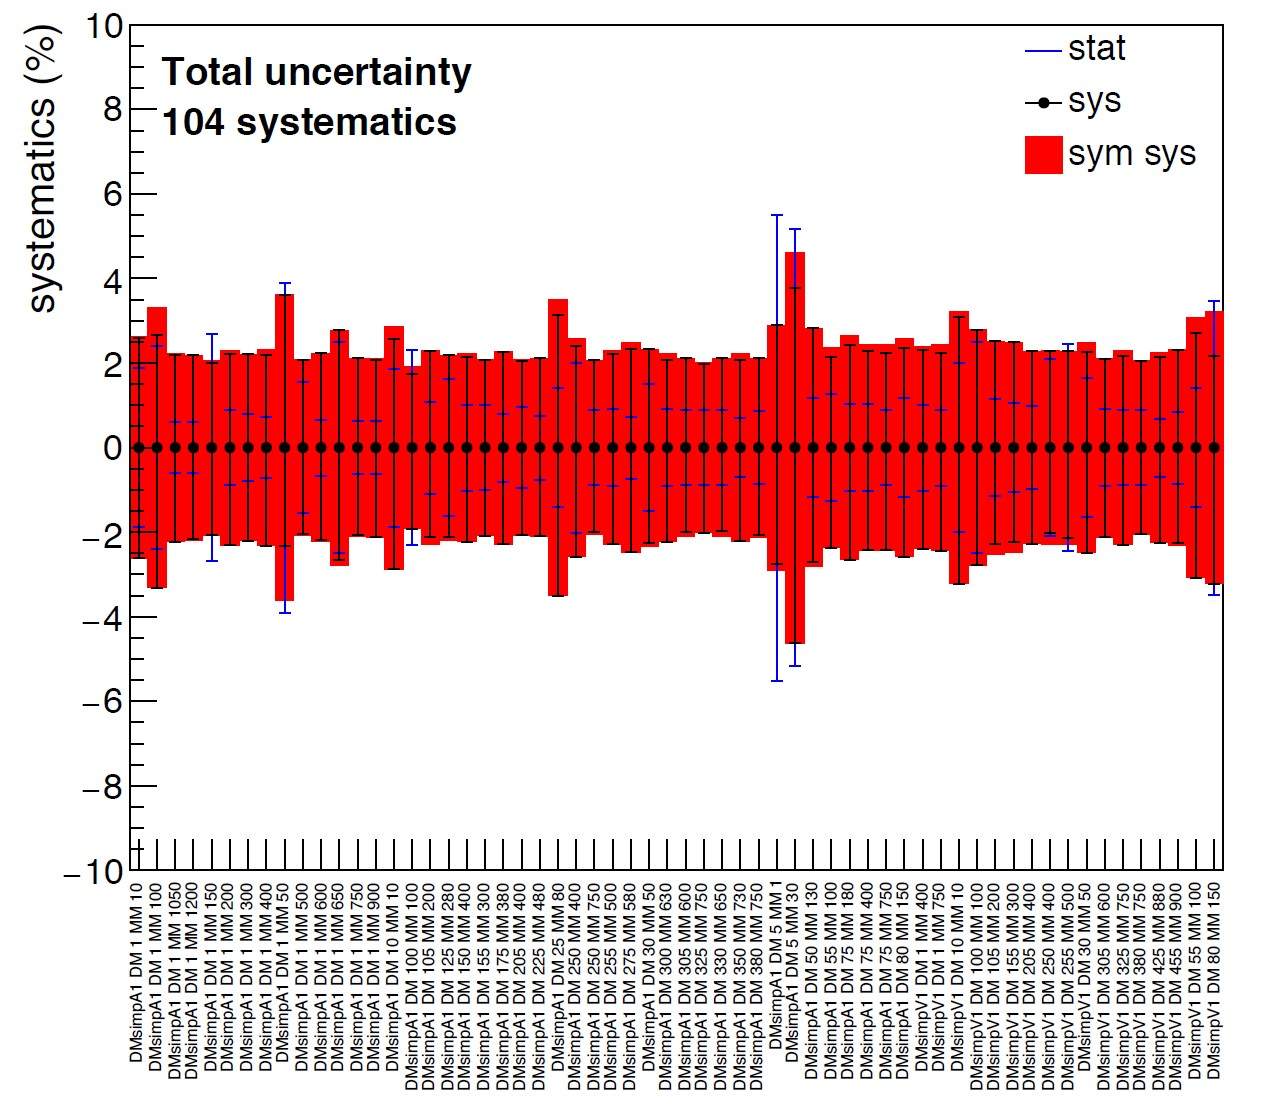
\includegraphics[width=0.8\linewidth]{figures/ch6-DM/ZHinv-syst-simplified-model.jpg}}\\
     \subfloat[]{
    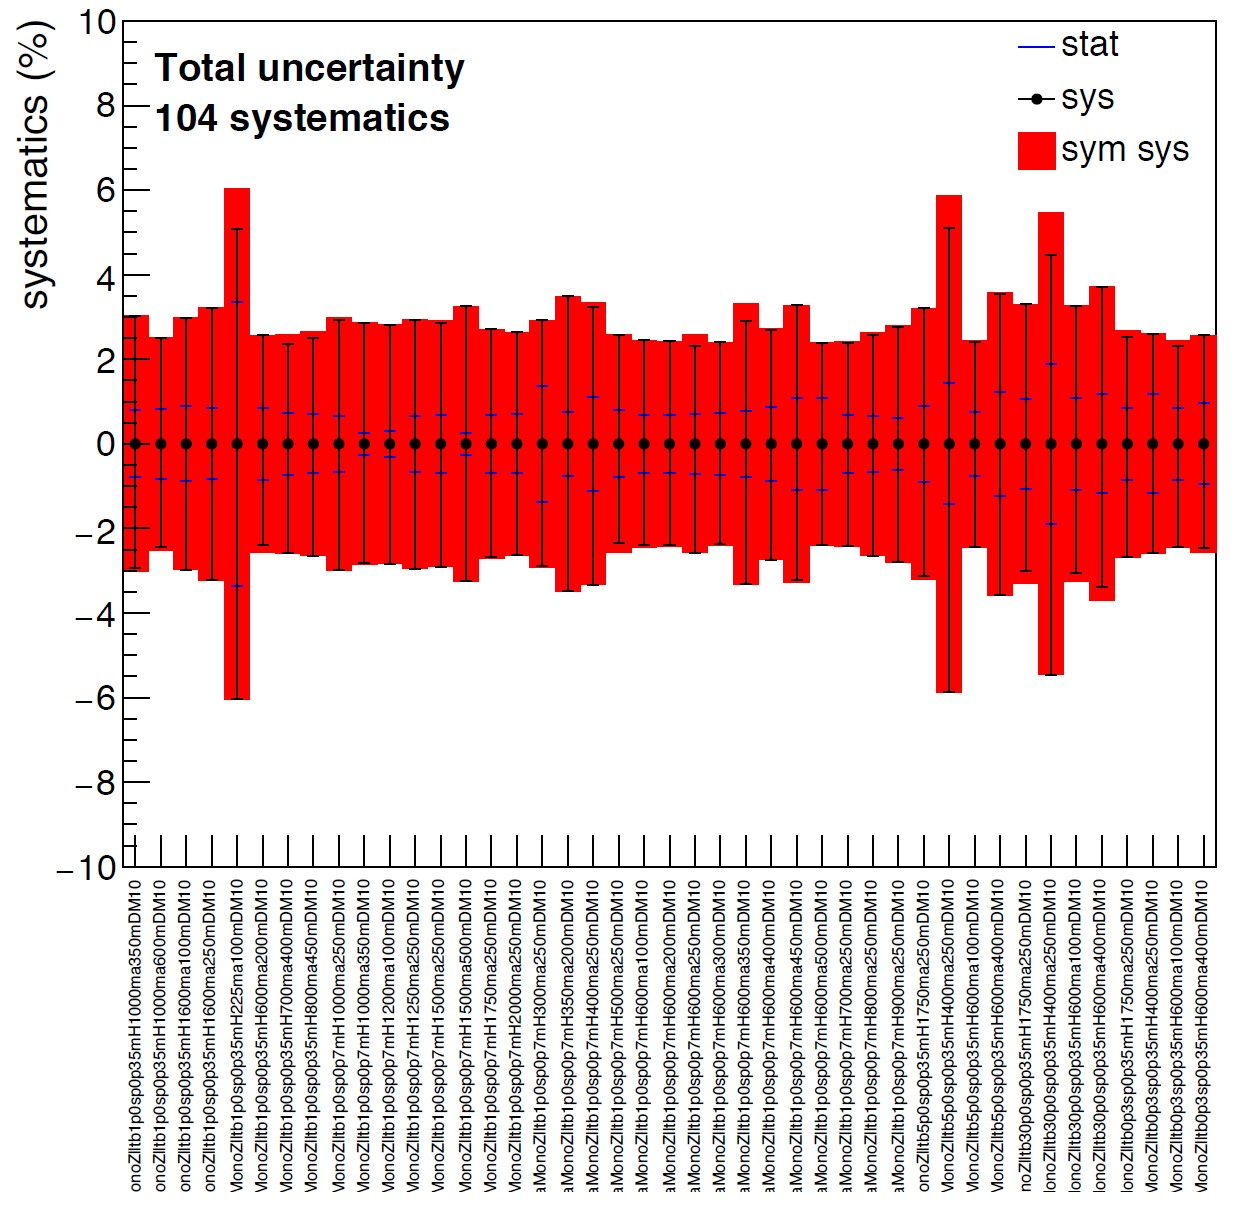
\includegraphics[width=0.8\linewidth]{figures/ch6-DM/ZHinv-syst-2HDMa.jpg}}
    \caption{\rm Summary of experimental uncertainties for all Mono-$\text{Z}$ (a) simplified model signal samples, and (b) 2HDM+$a$ samples.}
    \label{fig:MonoZ-syst-app}
\end{figure}

Figure~\ref{fig:pull-fit-app} shows the pulls of the nuisance parameters from the combined fit to data in the signal and control regions using the \textsc{HistFitter} framework. All nuisance parameters are well-behaved and constrained within their $\pm 1\sigma$ pre-fit expectations, demonstrating the stability of the background estimation and uncertainty modeling described in Section~\ref{sec:monoZ_results}.

\begin{figure}[htbp]
    \centering
    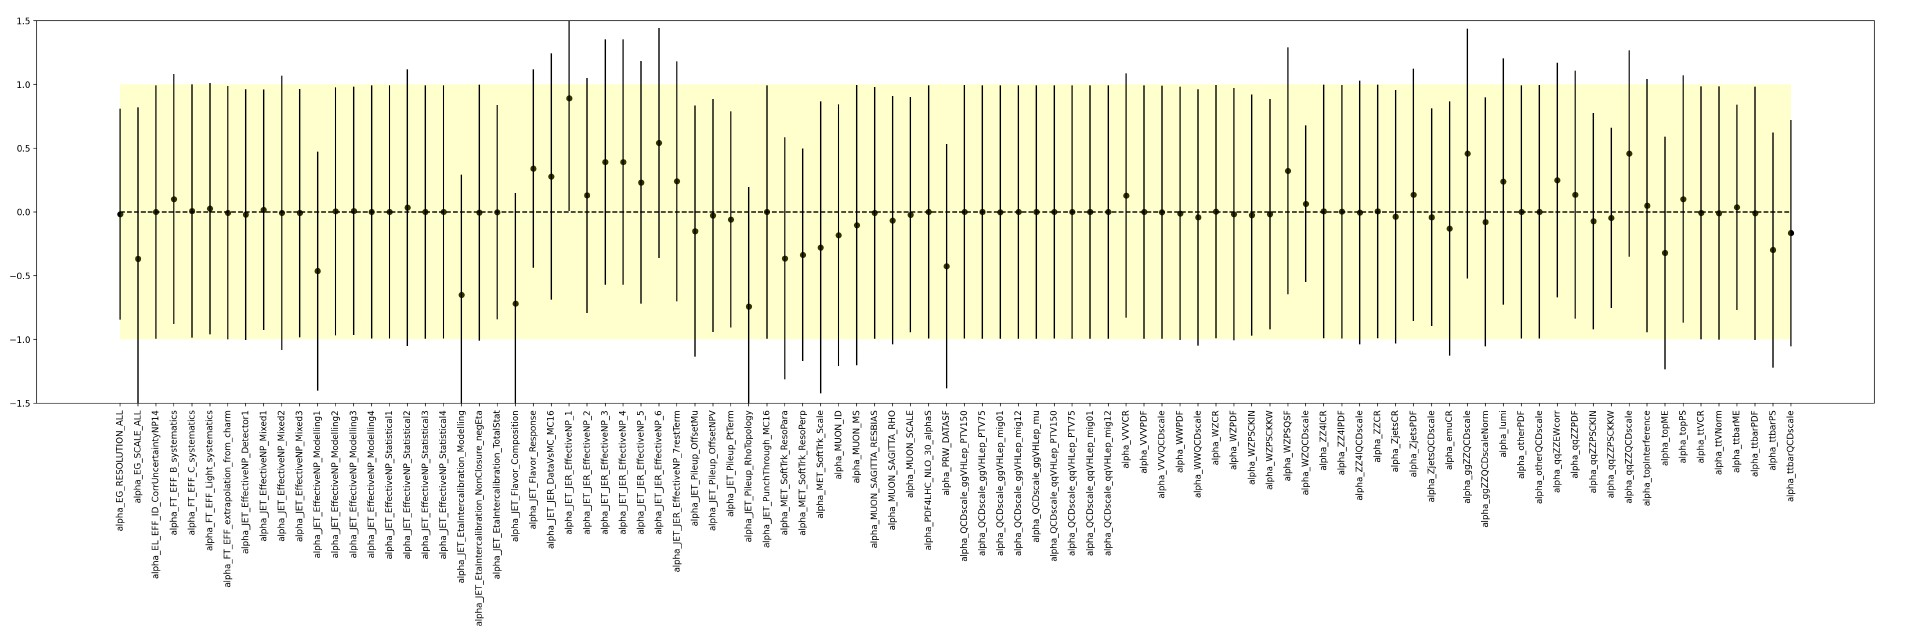
\includegraphics[width=0.98\linewidth]{figures/ch6-DM/ZHinv-fit-pull.jpg}
    \caption{\rm Pulls of the nuisance parameters from the combined fit to data.}
    \label{fig:pull-fit-app}
\end{figure}





